\documentclass[12pt,a4paper]{article}
\usepackage[UTF8]{ctex}
\usepackage{amsmath,amssymb}
\usepackage{tikz}
\usetikzlibrary{quantikz2}
\usepackage{listings}
\usepackage{xcolor}
\usepackage{hyperref}
\usepackage{geometry}
\geometry{margin=2.5cm}

\lstdefinestyle{python}{
  language=Python,
  basicstyle=\ttfamily\small,
  keywordstyle=\color{blue}\bfseries,
  commentstyle=\color{gray},
  stringstyle=\color{red},
  showstringspaces=false,
  breaklines=true,
  frame=single,
  backgroundcolor=\color{gray!10}
}

\title{Bell State / Bell 态}
\author{QuoNic}
\date{}

\begin{document}
\maketitle

\begin{center}
\textbf{Foundational / 基础} | 难度：初级 | 预计时间：5 分钟
\end{center}

\tableofcontents
\newpage

%% ============================================================
\section{为什么需要？}

在经典物理中，两个物体的状态是独立的——测量一个不会影响另一个。
但在量子世界中，两个量子比特可以进入一种\textbf{纠缠态}：测量其中一个，\textbf{瞬间}确定另一个的状态。

\subsection{经典局限}
\b\begin{itemize}
  \item 经典物理无法创建这种"超距关联"
  \item 经典通信需要至少 2 比特才能传输 1 比特量子信息
\end{itemize}

\subsection{量子优势}
\b\begin{itemize}
  \item Bell 态是量子纠缠的最基本形式
  \item 违反 Bell 不等式，证明量子力学是非局域的
  \item 是量子隐形传态、超密编码、量子密钥分发的基础
\end{itemize}

\subsection{实际应用}
\b\begin{itemize}
  \item 量子密钥分发（BB84、E91 协议）
  \item 量子隐形传态（量子网络的基础）
  \item 量子计算中的纠缠资源
\end{itemize}

%% ============================================================
\section{快速上手}

\begin{lstlisting}[style=python]
from quonic import qgate, qshow
from quonic.gates import CX, H

# 创建 Bell 态
qgate(H, 0)      # Hadamard 门：创建叠加态
qgate(CX, 0, 1)  # CNOT 门：创建纠缠
qshow()           # 测量并显示结果
\end{lstlisting}

\textbf{预期输出}：
\begin{verbatim}
backend: native | shots: 1024
Result:
  |00>     512  ( 50.0%)  ####################
  |11>     512  ( 50.0%)  ####################
\end{verbatim}

%% ============================================================
\section{原理详解}

\subsection{电路图}

\begin{center}
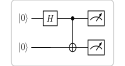
\includegraphics[width=0.6\textwidth]{../../images/bell_circuit_new.svg}
\end{center}

\subsection{数学推导}

\textbf{Step 1: 初始状态}

两个量子比特都从 $|0\rangle$ 开始：
\begin{equation}
|\psi_0\rangle = |00\rangle
\end{equation}

\textbf{Step 2: Hadamard 门}

对 $q_0$ 施加 $H$ 门：
\begin{equation}
H|0\rangle = \frac{|0\rangle + |1\rangle}{\sqrt{2}}
\end{equation}

所以状态变为：
\begin{equation}
|\psi_1\rangle = \frac{|0\rangle + |1\rangle}{\sqrt{2}} \otimes |0\rangle = \frac{|00\rangle + |10\rangle}{\sqrt{2}}
\end{equation}

\textbf{Step 3: CNOT 门}

CNOT 门的规则：如果控制比特是 $|1\rangle$，就翻转目标比特。
\begin{align}
\text{CNOT}|00\rangle &= |00\rangle \\
\text{CNOT}|10\rangle &= |11\rangle
\end{align}

所以最终状态：
\begin{equation}
|\psi_2\rangle = \frac{|00\rangle + |11\rangle}{\sqrt{2}}
\end{equation}

\textbf{Step 4: 测量概率}

测量时：
\b\begin{itemize}
  \item $P(|00\rangle) = |1/\sqrt{2}|^2 = 0.5$
  \item $P(|11\rangle) = |1/\sqrt{2}|^2 = 0.5$
  \item $P(|01\rangle) = 0$
  \item $P(|10\rangle) = 0$
\end{itemize}

\subsection{几何解释}

在 Bloch 球上：
\b\begin{itemize}
  \item $|0\rangle$ 在北极
  \item $|1\rangle$ 在南极
  \item $H$ 门把 $|0\rangle$ 旋转到赤道上的 $|+\rangle = (|0\rangle+|1\rangle)/\sqrt{2}$
\end{itemize}

CNOT 门创建纠缠后，两个量子比特的状态不再能用单个 Bloch 球描述——它们成为一个整体，这就是纠缠的几何意义。

%% ============================================================
\section{代码详解}

\begin{lstlisting}[style=python]
from quonic import qgate, qshow  # 导入核心 API
from quonic.gates import CX, H   # 导入门定义

# qgate(gate, qubit) —— 对指定量子比特施加门
qgate(H, 0)      # 对 q0 施加 Hadamard 门
                  # H 门作用：|0> -> (|0>+|1>)/sqrt(2)
                  # 效果：创建叠加态

# qgate(gate, control, target) —— 对两个量子比特施加受控门
qgate(CX, 0, 1)  # CNOT 门：控制=q0，目标=q1
                  # 作用：如果 q0 是 |1>，就翻转 q1
                  # 效果：创建纠缠态 (|00>+|11>)/sqrt(2)

# qshow() —— 运行电路并显示结果
qshow()           # 自动选择最佳后端
                  # 执行 1024 次测量
                  # 显示测量结果的统计分布
\end{lstlisting}

\subsection{API 说明}

\begin{center}
\begin{tabular}{|l|l|l|}
\hline
\textbf{API} & \textbf{参数} & \textbf{说明} \\
\hline
\texttt{qgate(H, 0)} & H: Hadamard 门, 0: 量子比特索引 & 对 $q_0$ 施加 $H$ 门 \\
\hline
\texttt{qgate(CX, 0, 1)} & CX: CNOT 门, 0: 控制比特, 1: 目标比特 & 创建纠缠 \\
\hline
\texttt{qshow()} & 无参数 & 运行电路并显示结果 \\
\hline
\end{tabular}
\end{center}

%% ============================================================
\section{进阶用法}

\subsection{场景 1：创建不同 Bell 态}

\begin{lstlisting}[style=python]
# Phi+ = (|00>+|11>)/sqrt(2)
qgate(H, 0)
qgate(CX, 0, 1)

# Phi- = (|00>-|11>)/sqrt(2)
qgate(H, 0)
qgate(X, 0)  # 相位翻转
qgate(CX, 0, 1)

# Psi+ = (|01>+|10>)/sqrt(2)
qgate(H, 0)
qgate(CX, 0, 1)
qgate(X, 1)  # 翻转 q1

# Psi- = (|01>-|10>)/sqrt(2)
qgate(H, 0)
qgate(X, 0)
qgate(CX, 0, 1)
qgate(X, 1)
\end{lstlisting}

\subsection{场景 2：多量子比特 GHZ 态}

\begin{lstlisting}[style=python]
# GHZ 态：(|000>+|111>)/sqrt(2)
qgate(H, 0)
qgate(CX, 0, 1)
qgate(CX, 1, 2)
qshow()
\end{lstlisting}

\subsection{场景 3：噪声下的 Bell 态}

\begin{lstlisting}[style=python]
# 无噪声
qshow(noise=0)

# 5% 噪声
qshow(noise=0.05)

# 20% 噪声
qshow(noise=0.20)
\end{lstlisting}

%% ============================================================
\section{适用场景}

\subsection{量子密钥分发}

BB84 和 E91 协议使用 Bell 态来检测窃听。如果有人试图测量量子态，就会破坏纠缠，通信双方可以检测到。

\subsection{量子隐形传态}

量子隐形传态使用 Bell 态作为量子信道，可以在不直接传输量子比特的情况下传输量子态。

\subsection{量子计算测试}

Bell 态是测试量子硬件质量的金标准。如果硬件不能正确制备 Bell 态，说明有噪声或校准问题。

%% ============================================================
\section{常见问题}

\subsection{为什么我的结果不是精确的 50/50？}

量子测量有随机性。即使理论概率是 50/50，有限次测量（如 1024 次）也会有统计涨落。增加 shots 数量可以更接近理论值。

\subsection{为什么我看到了 |01> 或 |10>？}

可能原因：
\begin{enumerate}
  \item 噪声（检查是否设置了 noise 参数）
  \item 代码错误（确认 H 门在 CNOT 之前）
  \item 后端问题（试试 \texttt{backend='native'}）
\end{enumerate}

\subsection{Bell 态和 GHZ 态有什么区别？}

Bell 态是 2 量子比特纠缠，GHZ 态是 3+ 量子比特纠缠。GHZ 态是 Bell 态的推广，用于多方量子通信和量子纠错。

\subsection{如何验证我制备的是 Bell 态？}

检查测量结果：
\begin{enumerate}
  \item 只有 $|00\rangle$ 和 $|11\rangle$
  \item 两者概率接近 50\%
  \item 没有 $|01\rangle$ 和 $|10\rangle$
\end{enumerate}
如果满足这三个条件，就是 Bell 态。

\subsection{Bell 态违反 Bell 不等式是什么意思？}

经典物理中，两个粒子的关联有一个上限（Bell 不等式）。量子力学的预测超过这个上限，实验证实了量子力学的正确性。这意味着没有局域隐变量理论能解释量子关联。

%% ============================================================
\section{学习路径}

\subsection{前置知识}
\b\begin{itemize}
  \item 量子比特的基本概念（$|0\rangle$ 和 $|1\rangle$）
  \item 叠加态和 Hadamard 门
  \item CNOT 门的作用
\end{itemize}

\subsection{继续学习}
\b\begin{itemize}
  \item 量子隐形传态（使用 Bell 态传输量子态）
  \item 超密编码（使用 Bell 态传输经典信息）
  \item GHZ 态（多量子比特纠缠）
\end{itemize}

\subsection{难度等级}
\b\begin{itemize}
  \item 当前：初级
  \item 下一步：中级
\end{itemize}

%% ============================================================
\section{完整示例代码}

\subsection{示例 1：基本 Bell 态}

\begin{lstlisting}[style=python]
from quonic import qgate, qshow
from quonic.gates import CX, H

qgate(H, 0)
qgate(CX, 0, 1)
qshow()
\end{lstlisting}

\subsection{示例 2：带噪声的 Bell 态}

\begin{lstlisting}[style=python]
from quonic import qgate, qshow
from quonic.gates import CX, H

qgate(H, 0)
qgate(CX, 0, 1)
qshow(noise=0.05)
\end{lstlisting}

\subsection{运行方式}

\begin{verbatim}
python examples/bell/bell.py
\end{verbatim}

\

\section{下载}

\begin{itemize}
  \item [bell.py](https://github.com/ChrisLee0721/QuoNic/blob/main/examples/bell/bell.py)
\end{itemize}

\end{document}
